% !TEX root = poster.tex
\headerbox{\textbf{Basics}}{name=basics,column=0, row=0}{
\textbf{Introduction}\\[0.5em]
Measurements of flavour oscillations and time-dependent \CP asymmetries in neutral $B$ meson systems require knowledge of the $b$ quark flavour at production. This identification is performed by the Flavour Tagging (FT). [1,2]\\[0.8em]
%Knowledge of $b$ quark production flavours is crucial for measurements of flavour oscillations and time-dependent \CP asymmetries in neutral \B meson systems. At LHCb this identification is performed by the Flavour Tagging. [1]\\[0.9em]
\textbf{Two independent classes of algorithms}
\vspace{-0.5em}
\begin{itemize}
\item \textbf{same side taggers (SS)}\\[0.06cm]
%use the particle accompanying the fragmentation of the \bquark quark producing the signal \B meson
use charged particles created in the fragmentation process of the \bquark quark of the signal \B meson
\vspace{-0.59em}
\begin{itemize}
\setlength\itemsep{0.01em}
\setlength{\itemindent}{-.11in}
\item[${\color{tu_gruen}-}$] kaon for \Bs  \hspace{2.455em} ${\color{tu_gruen}\rightarrow}$ SS kaon / SS kaon nnet
\item[${\color{tu_gruen}-}$] pion for \Bd \quad \qquad ${\color{tu_gruen}\rightarrow}$ SS pion 
\item[${\color{tu_gruen}-}$] proton for \Bd \qquad ${\color{tu_gruen}\rightarrow}$ SS proton
\end{itemize}
\vspace{-0.6em}
\item \textbf{opposite side taggers (OS)}\\
exploit the non-signal \bquark quark of the initial \bbbar pair
\vspace{-0.55em}
\begin{itemize}
\setlength\itemsep{0.01em}
\setlength{\itemindent}{-.11in}
\item[${\color{tu_gruen}-}$] overall charge of the secondary vertex (SV) \\ ${\color{tu_gruen}\rightarrow}$ OS vertex charge
\item[${\color{tu_gruen}-}$] lepton from semi-leptonic $b$ hadron decays \\ ${\color{tu_gruen}\rightarrow}$ OS muon / OS electron
\item[${\color{tu_gruen}-}$] kaon from the \bquark$\rightarrow$\cquark$\rightarrow$\squark decay chain \\ ${\color{tu_gruen}\rightarrow}$ OS kaon 
\item[${\color{tu_gruen}-}$] \D meson from the \bquark$\rightarrow$\cquark decay chain \\ ${\color{tu_gruen}\rightarrow}$ OS charm (New!)
\end{itemize}
\end{itemize}
\begin{center}
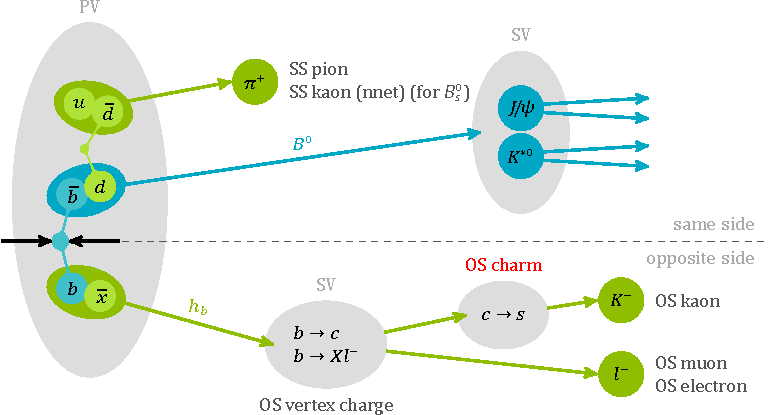
\includegraphics[width=\textwidth]{FTScheme/FlavourTaggerScheme.pdf}
\end{center}
\vspace{-0.6em}
Each tagger provides a decision $d$ on the initial flavour \newline(“tag”) and a probability to be wrong,  $\eta$.\\[0.3cm]
%\begin{itemize}
%\setlength\itemsep{0.01em}
%\item a decision on the initial flavour ("tag")
%\item an estimate to be wrong ($\eta$)
%\end{itemize}
\vspace{-0.75em}
\textbf{Flavour Tagging characteristics}
\vspace{0.1em}
\begin{itemize}
\item \textbf{mistag} \\[0.04cm] 
fraction of events with a wrong tagging decision
\begin{equation*}
\hspace{-1.6em}
\omega=\frac{N_{\text{wrong}}}{N_{\text{right}}+N_{\text{wrong}}}
\end{equation*}
\vspace{-1.1em}
\item \textbf{tagging efficiency} \\[0.04cm] 
fraction of events with a tagging decision
\begin{equation*}
\hspace{-1.6em}
\varepsilon_\text{tag}=\frac{N_{\text{right}}+N_{\text{wrong}}}{N_{\text{all}}}
\end{equation*}
\vspace{-1.1em}
\item \textbf{effective tagging efficiency} \\[0.04cm] 
represents the statistical reduction factor of a sample in a tagged analysis
\vspace{-0.3em}
\begin{equation*}
\hspace{-1.6em}
\vspace{0.5em}
\varepsilon_\text{eff}=\varepsilon_\text{tag}\left(1-2\omega\right)^2
\end{equation*}
\end{itemize}
%$N_R$/$N_W$/$N_U$ $:=$ number of correctly/incorrectly/untagged events.
%where $R$,$W$,$U$ are the number of correctly tagged, incorrectly tagged and untagged events. The tagging algorithms were developed and studied simulated events. (??) (REF)\\


}
